\chapter{Modular architecture}
\label{sec:ModularArchitecture}

A modular architecture:
\largequote{Modular design or “modularity in design” is a design approach that subdivides a system into smaller parts called modules or skids that can be independently created and then used in different systems. A modular system is characterized by functional partitioning into discrete scalable and reusable modules, rigorous use of well-defined modular interfaces and making use of industry standards for interfaces. \cite{whatIsModularArchitecture}}

When researching famous architectures in software there are a few examples of non modular architectures. Such an architecture is the layered architecture. In the image below is shown how such an architecture operates.

\begin{figure}[H]
	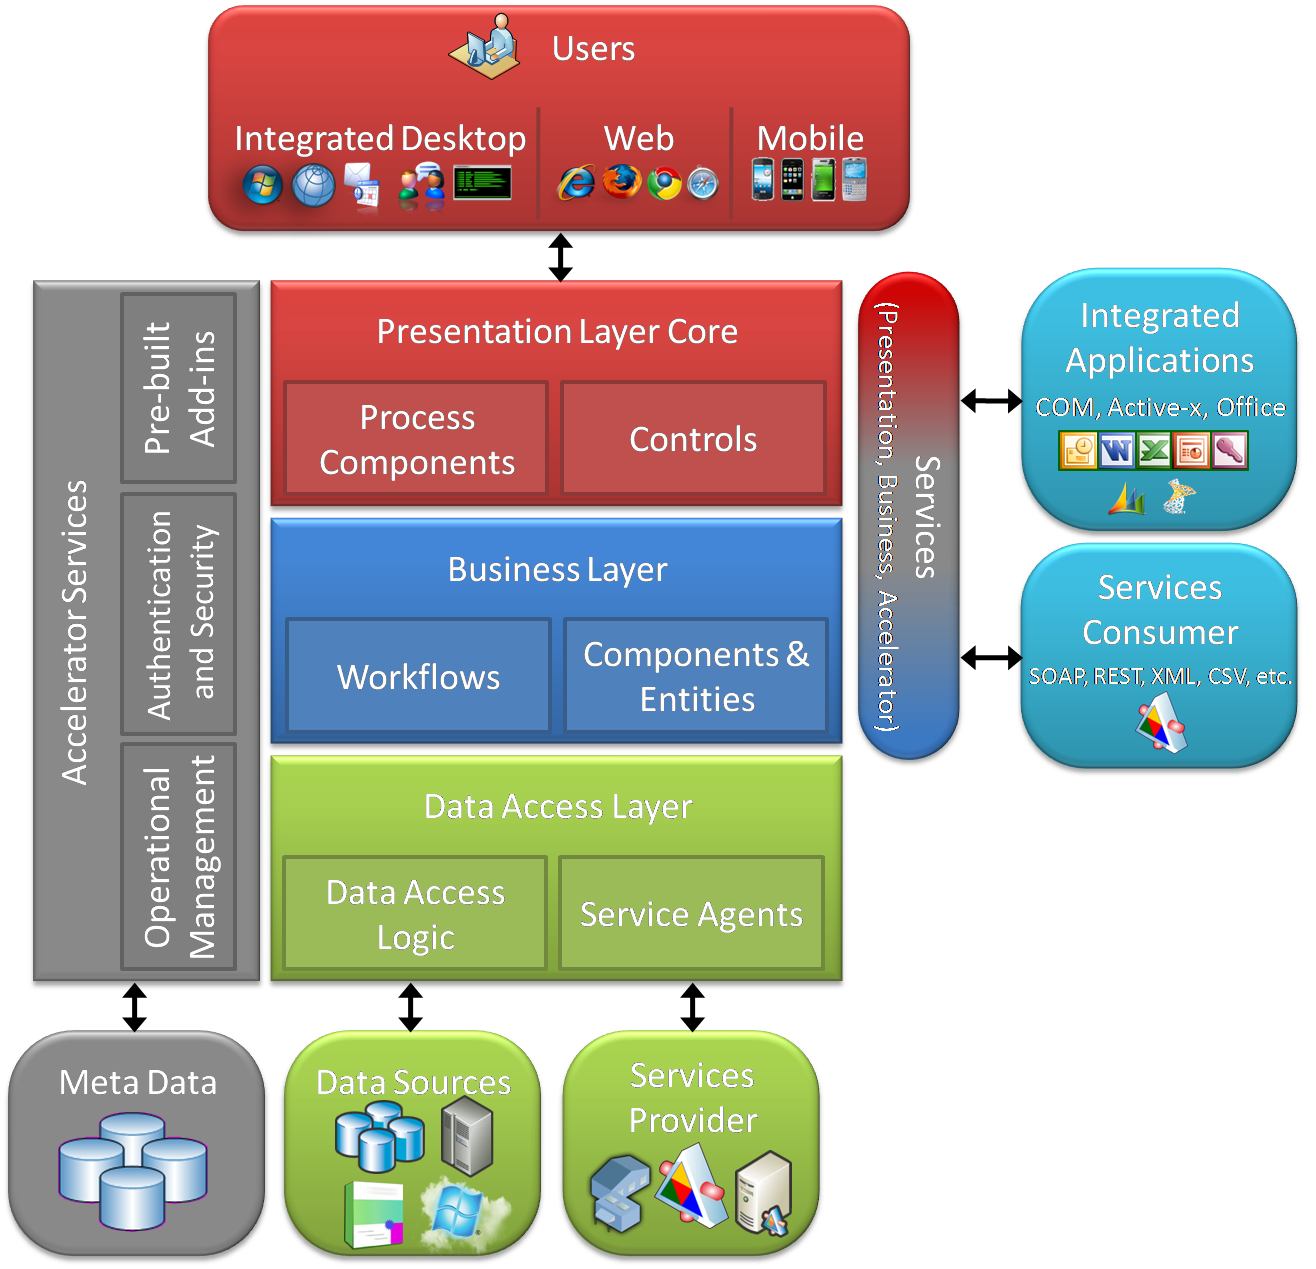
\includegraphics[width=\linewidth]{layered_architecture.png}
	\caption{Layered architecture \cite{layeredArchitecture}}
\end{figure}

As shown in the figure the architecture is layered based on responsibilities. Each layer having its own purpose. The layers can talk with each other but they are intertwined. This means that a class or object in the presentation layer can talk to the same business layer object as another presentation layer class. This concludes in the objects being highly coupled.

A modular architecture is based upon modules. A module is:
\largequote{deployable, manageable, natively reusable, composable, stateless unit of software thatprovides a concise interface to consumers” \cite{moduleDefinition}}

This is eerily similar as the description of what this research calls building blocks in \fullref{sec:TheProblem}

\section{Architectures}
\label{sec:Architectures}

\subsection{Microservices}
If most software engineers in 2019 think of a modular software architecture the first architecture that comes to mind is microservices. In the last years microservices have seen a surge in usage. One of the biggest companies that showed its effectiveness is Netflix \cite{microservicesNetflix}.

\subsubsection{Definition}
The best way to describe a microservice is:
\largequote{A particular way of designing software applications as suites of independently
deployable services. \cite{microservicesDefinition}}

While there is no concrete definition of a microservice there are some characteristics that
every definition contains.
\begin{itemize}
        \item \textbf{Highly maintainable and testable:} enables rapid and frequent development and deployment

        \item \textbf{Loosely coupled with other services:} enables a team to work independently the majority of time on their service(s) without being impacted by changes to other services and without affecting other services

        \item \textbf{Independently deployable:} enables a team to deploy their service without having to coordinate with other teams

        \item \textbf{Capable of being developed by a small team:} essential for high productivity by avoiding the high communication head of large teams \cite{microservicesCharactaristics}
\end{itemize}

Now that there is a clear understanding of what microservices are and which principles
they should follow. Some best practices can be pinpointed.

\subsubsection{Best practices}
The first best practices is to \textbf{create a seperate datastore} for each microservice. First of all not every datastore fits every service. It may be that a message service may achieve more efficiency from a NoSQL database and a user service from an SQL database. A benefit stemming from this is that microservices lets the team think about each datastore used for each service and why that datastore is the correct one for that specific service \cite{microservicesNetflix}.

When creating a separate datastore for each service you run the risk of data inconsistency. For example, there is a user service which stores the user id. There is also a message service which stores the message and the user id to whom the message is send. If a user gets deleted in the user service, this should reflect in the message service. But with microservices this is not automatically the case because each service has its own datastore. Therefore the foreign keys are not native and thus will not be updated or give a warning.

Another best practice is \textbf{writing documentation} \cite{microservicesBestPractice} for each microservice. Most importantly about how they should be used and which interface it uses. For example, when a new service is created next to our messaging and user service called file service which handles the files send in the messages. This service should know how to communicate with the message service. This makes it easier for the new services to connect to the existing services.

Another challenge with microservice is the \textbf{monitoring} \cite{microservicesBestPractice} of the services. Because it is not known how many services are online it is important to know when they are online and what they log. For example, our messaging service is used frequently and duplicates itself. This then means that the logging of the new service needs to be picked up by your monitoring system in order to view the whole picture of the running application.

\subsection{Miniservices}
One of the “new” ones is miniservices. The reason new is between quotes is because most companies that implement microservices actually implement miniservices. The difference between microservices and miniservices is best described in the figure below:

\begin{figure}[H]
	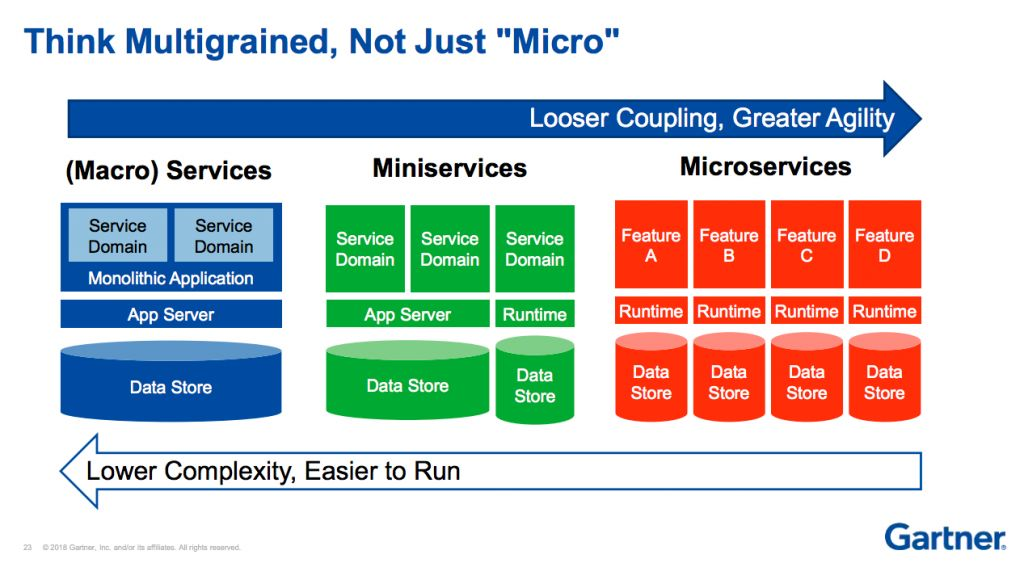
\includegraphics[width=\linewidth]{miniservices.png}
	\caption{Miniservices architecture \cite{miniservicesDefinition}}
\end{figure}

Miniservices is essentially an architecture based on breaking specific rules of microservices \cite{miniservicesOrigin}. As shown in the picture the biggest difference between microservices and miniservices is that microservices are actual features being decoupled and miniservice is about decoupling a domain of features.

This means that each service may contain multiple features but all of the features should be linked to the same domain. Thus the communication inside a service is more fluent and needs less network design than microservices does.

Another divergence is that each microservice should have a separate datastore. This is not the case for miniservices. Every miniservice may be connected with the same datastore \cite{miniservicesDefinition}.

The main advantage miniservices has over microservices is the complexity of the network architecture. With microservices every service is singled out. Which means no service knows about each other so the protocol in which the services speak can be different and may differ from service to service. With miniservices each service connects to the same database. Which makes it easier and faster to do complex querying.

\subsection{Modular monolith}
\label{sec:ModularMonolith}

The main idea behind a modular monolith is preserving the idea of encapsulation but deploying it differently \cite{modularMonolithIdea}. Instead of deploying different services separately with each service having its own datastore, a module can be a library, plugin or namespace. This makes deploying easier to manage whilst still having the modularity gotten from encapsulation.

Just like with miniservices each module will contain the functionalities of a single domain. But unlike the miniservices the modular monolith is compiled to one application instead of multiple.

Modular monolith is perfect for smaller teams because it does not require as much setup as miniservices or microservices.

\section{The comparison}
\label{sec:Comparison}

A good talk about modular monoliths \cite{modularMonolithTalk} shows that most of the time when thinking of architecture there are two extremes. The monoliths and the microservices. As shown in the figure below:
\begin{figure}[H]
	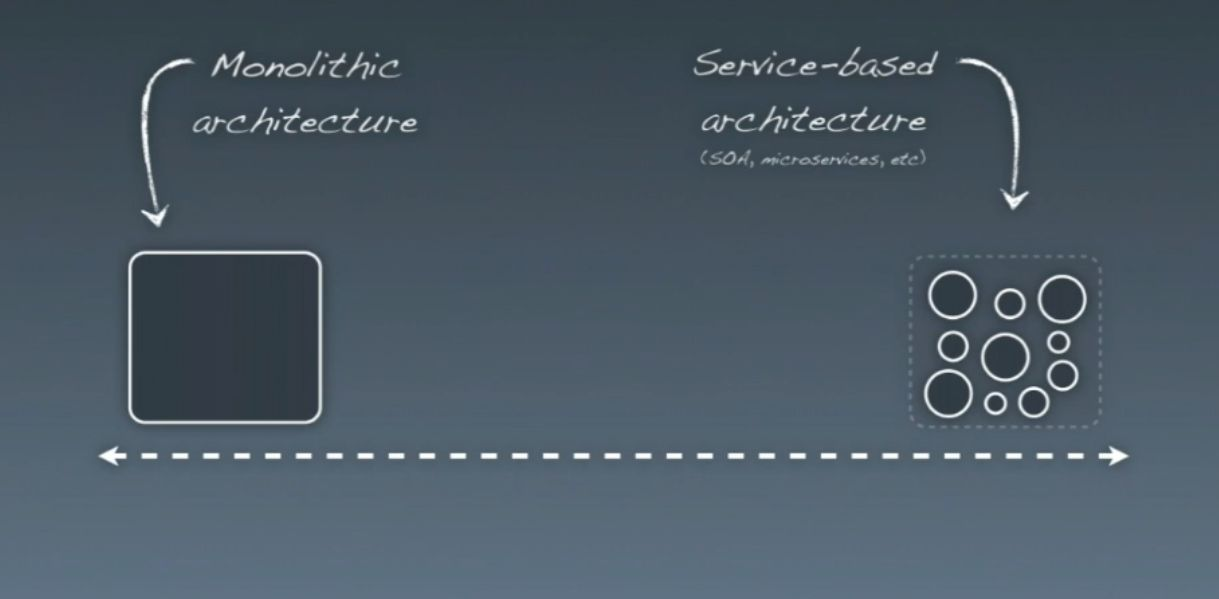
\includegraphics[width=\linewidth]{microservices-spectrum.png}
	\caption{Monolith, microservices spectrum \cite{modularMonolithTalk}}
\end{figure}

But this is not always the case as shown in \fullref{sec:Architectures}.There are cases where microservices are the best choice and there are cases where miniservices or a modular monolith is the best choice. This chapter will further compare the three architectures and decide which architecture fits best with EFFE's priorities. This will be done with the help of chapter \fullref{sec:Priorities}

\section{Complexity}
\label{sec:Complexity}

Complexity always plays a role when choosing the right architecture. Looking at the three architectures shown in \fullref{sec:Architectures} it is obvious that the complexity changes the smaller the modules. Thus the most complex architecture is microservices and the least complex one is modular monolith. With miniservices right in the middle.

In the figure shown below there is an example of the microservice architecture. This shows that each service may have its own datastore but can also run on a different server. This means that each service needs to know in some way where the other services are located. This is called service discovery. Service instances have dynamically assigned network locations. Moreover, the set of service instances changes dynamically because of autoscaling, failures, and upgrades. Consequently, your client code needs to use a more elaborate service discovery mechanism \cite{serviceDiscovery}. This is also the case with miniservices.

\begin{figure}[H]
	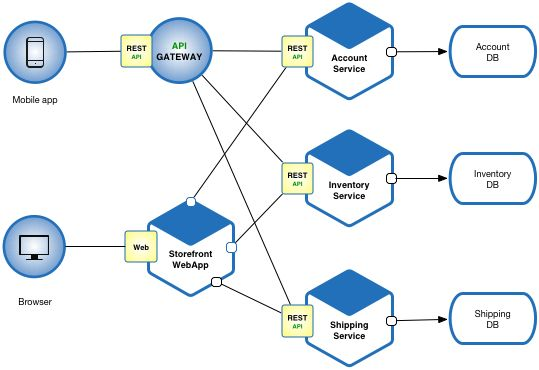
\includegraphics[width=\linewidth]{microservice-architecture.png}
	\caption{Microservice architecture}
\end{figure}

Even though they can connect to a centralized datastore the services do not have any knowledge of each other. In a monolitic application there are no different services. The modules can talk with each other via functions and imports. This means that there is knowledge of the other modules.

The other thing that makes microservices especially complex is the splitted datastores. Because the database is splitted it can be hard to handle foreign keys or pointers to other data objects. This is because the datastore does not have a direct connection to this pointer. This problem of complexity is not prevalent amongst the miniservices and modular monolith because in these architectures the datastore is shared.

The quality attributes that are applicable to this attribute are:
\begin{itemize}
        \item \textbf{Maintainability:} The more complex an infrastructure and/or architecture is the more maintenance it requires.
        \item \textbf{Security:} Complexity always brings security issues with itself. This is especially the case with miniservices and microservices because of the service discovery.
\end{itemize}

\section{Technology}
\label{sec:Technology}

One of the most convincing arguments for choosing microservices is the freedom of choosing the technology. There is a possiblity to write the first service with Node.js and a MongoDB database and the next service with Java and an ElasticSearch datastore. This makes it really easy when switching technology or recruiting new developers.

Miniservices does have the benefit of choosing a different programming language per service. But because all of the services talk with the same datastore, the datastore technology is always the same.

Modular monolith is the worst in this section. A modular monolith is stuck with the same technology for the programming language and the datastore.

The quality attributes that are relevant are:
\begin{itemize}
        \item \textbf{Porability:} The portability is very high because each service can be ported separately which makes it easier.
        \item \textbf{Compatability:} The compatibility between technologies is extremely relevant when looking at the architecture
        \item \textbf{Performance:} Because the technology for each service can be different. A language can be chosen to create the optimal performance for that specific service.
\end{itemize}

\section{Testing}
\label{sec:Testing}

It is known that testing plays a big role in creating reliable software. There are multiple types of testing \cite{testTypes}. Not all of them are useful for EFFE. That is why EFFE has created a list of tests it does on the current application. These are test types that will be looked at:

\begin{itemize}
        \item Unit tests
        \item Integration tests
        \item End-to-end tests
        \item Load tests
\end{itemize}

Each section will begin with a rating from 1 to 3 where 1 is the best architecture for this kind of test.

\subsection{Unit tests}
\label{sec:UnitTests}

\begin{enumerate}
        \item Microservices
        \item Miniservices
        \item Modular monolith
\end{enumerate}

In a microservice each function is its own service. So the functions are really easy to test. Because miniservices is domain based it takes a bit more effort to test the whole service but it is easier than the modular monolith. This is because the modular monolith is more tightly coupled than miniservices.

\subsection{Integration tests}
\label{sec:IntegrationTests}

\begin{enumerate}
        \item Modular monolith
        \item Miniservices
        \item Microservices
\end{enumerate}

Because the modular monolith contains all its services it is easy to test how they work together. This can even be done with unittesting. For the miniservices and microservices it is more difficult. The reasoning behind this is the complexity of the service discovery. To test for example two services, service discovery needs to be setup. Each extra service that is added to the tests will add more complexity. An integration test with microservices may call six different services. But with miniservices it may be less if the functions that are called are in the same domain. This is why microservices is in the last place in this type of testing.

\subsection{End-to-end tests}

\begin{enumerate}
        \item Modular monolith
        \item Miniservices
        \item Microservices
\end{enumerate}

As seen in the \fullref{sec:IntegrationTests} the same type of problem occurs. A function that is called may need multiple microservices or miniservices called.

\subsection{Load tests}

No difference

All of the architectures are equal when it comes to load testing. This is because load testing is done on a live site. This does not mean it has to be done on production, although it can be.

\subsection{Conclusion}

The quality attributes that testing influences are:

\begin{itemize}
        \item \textbf{Maintainability:} Unit testing and integration testing creates an environment that gives the developer a guideline he or she should follow. The developer knows what is expected and thus can maintain the application with more ease.

        \item \textbf{Compatibility:} Almost all of the test types look at if the code works and will fail if it changes. The backwards compatibility Of a application will be tested constantly.

        \item \textbf{Functional sustainability:} This is where testing started. Writing unit tests to be sure the functionality has not changes.

        \item \textbf{Performance:} With load testing performance will be tested this won’t be taken in consideration because there was no difference between the architectures.

        \item \textbf{Usability:} End-to-end testing is specifically made for testing usability. It checks if the UI of an application still behaves the same.
\end{itemize}

\section{Costs}
\label{sec:Costs}

Because EFFE is a startup costs are very important. EFFE does not have the steady money flow that a more mature company may have.

There are two parts on how costs are calculated for software. The first one contains the price of development and the second one is the price of hosting.

Development time and understanding the code go hand in hand. When a developer does not understand the code the developer can not develop. So how do these architectures hold up considering development time and understanding the code?

Microservices as mentioned before is a very complex architecture but when developing it is one of the easiest. Because each function is its own service, creating a service is really easy. There is not a great number of code in one function and therefore easy to understand.

Miniservices and a modular monolith are in the same situation the code can be more complex because they need to talk to other services or modules but there is also a great number of code in one service or module. Therefore understanding the code and the developing time become larger.

The difference between the architectures is not very big. If miniservices and modular monolith are structured in such a way that is logical it should not matter.

Modular monolith is by far the least expensive architecture. Because the application can run on one server without the expense of server discovery it can be run on a server that costs \$5,- a month \cite{digitalOcean}. But the tricky parts comes when talking about interchangeability. What happens if a company wants a building block changed slightly only for them. If they are willing to pay for it it means that there needs to be a whole new server because the application is build on its own. When EFFE has five clients who want this and five clients that run on the standard version. EFFE would have to run it on six servers which would be \$30 dollars on the cheapest server which is not expensive at all.

Microservices and miniservices are the opposite with microservices standing out more. These services require server discovery as mentioned before. There are open source server discovery services such as \href{https://www.consul.io/}{consul} but those also need a seperate server. Server discovery is not the most expensive part. The most expensive part is a combination of having multiple services running on different servers that can autoscale. This means that there is less knowledge about our spendings beforehand.

There are some amazing services that handle deployment and autoscaling for microservices. The most known are Kubernetes, Nomad and Docker swarm. These services however cost \$40,- per month with the minimum requirements. The cost of the servers and the orchestrator can ramp up quickly.

The quality attribute that is most affected by the cost is the \textbf{maintainability}. This is purely because if the infrastructure is this expensive there would be no money to maintain it.

Thus when looking at development time vs infrastructure costs there is a lot to say for the modular monolith. Because even tho the development time is a bit slower for modular monoliths the infrastructure is way cheaper than miniservices or microservices.

\section{Scalability}
\label{sec:Scalability}

It would not be fair to compare these architectures without taking a look at scalability. This is where microservices shine. Microservices are made for horizontal scaling.

Vertical scaling is when hardware resources are added to a server. For example adding 4GB of ram to a server. Horizontal scaling is when adding more instances of the service. This can be on multiple servers \cite{microservicesMultipleServer}.

As mentioned before microservices is created for horizontal scaling. When a service suddenly gets a lot of traffic the service can autoscale itself. This can be done rather easily because the service itself is so small. This is also why it is harder with miniservices and even harder with modular monolith.

Scalability is important when talking about \textbf{performance}. When a server is going above a certain threshold it can duplicate itself and can now split the traffic along the new instance.

\section{Frontend}
\label{sec:FrontendComparison}

When looking at the architecture there is one that stands out as easily adapted for frontend and that is modular monolith. This is because it will still be compiled to one application.

Right now EFFE uses Vue to create a single page application. But this does not mean other frontend frameworks are not considered explained in \fullref{sec:Frontend}.

When looking at microservices in the backend there is a similar phenomenon in the frontend called micro-frontend or micro-apps \cite{microFrontends}. But there is one problem that persists with this solution and that is the sharing of UI elements. There is an option to share them between services but that would mean each service would use the same language and need to be deployed all together if one of those UI elements change. Therefore this is not a solution. A talk about micro-apps (microservices frontend) gave a convincing story about why someone should switch to them \cite{frontendMicroservices}. But when asked about the UI elements there was no answer that fixed this problem.

Concluding that for frontend there is only one possibility for a modular architecture and that is modular monolith.

\section{Recap}

This is a recap of what is discussed in \fullref{sec:ModularArchitecture}. As mentioned in \fullref{sec:Comparison} in this research there will be looked at the quality attributes and how they matched up per architecture.

\fullref{sec:Complexity} talks about the complexity and how it can influence the whole project. The architecture that ended on top was modular monolith and the quality attributes that were applicable where \textbf{maintainability} and \textbf{security}.

In \fullref{sec:Technology} microservices came out on top. With miniservices following and modular monolith as an obvious last. The quality attributes that are influenced by technology are \textbf{compatibility}, \textbf{performance} and \textbf{portability}

\fullref{sec:Testing} was by far the most contested section with no clear winner. But when looking at the types of tests that were considered (unit, integration, end-to-end and load testing) modular monolith ended with the best result with miniservices again in the middle and microservices ending last. The quality attributes for testing are \textbf{maintainability}, \textbf{compatibility}, \textbf{funtional sustiainability}, \textbf{performance} and \textbf{sustainability}

In \fullref{sec:Costs} the clear winner is modular monolith with miniservices following and microservices at an obvious last place. The quality attribute affected by the cost is \textbf{maintainability}

\fullref{sec:Scalability} has microservices at first. In second place is miniservices and last is modular monolith. The quality attribute applicable is \textbf{performance}.

In \fullref{sec:FrontendComparison} there was eventually only one architecture that actually made sense and that was the modular monolith.

\section{Conclusion}

The architecture that fits EFFE best is the modular monolith. The chapters where modular monolith was the best option were also the ones that influenced the quality attribute \textbf{maintainability} the most. As sorted in \fullref{sec:IsoRecap} \textbf{maintainability} is by far the most important quality attribute for EFFE. EFFE also does not have much money as mentioned in \fullref{sec:Costs} Thus costs play a big part in this decision as well. Finally the modular monolith architecture is especially good for small teams and that is a perfect description of the software team of EFFE since it exists out of one person at the moment.

Microservices have the clear distinction of winning the race on technology and scalability but this is not where the focus of this research lays. Although technology aligns with some of EFFE's focusses it does not compete with the main focus that the modular monolith architecture touches on and the pros do not outweigh the cons.

Miniservices is a mixture of modular monolith and microservices and takes some good parts of the both architectures but also some drawbacks of both architectures. The biggest downside is the complexity of the network as explained in \fullref{sec:Complexity}.
